การติดตามการเคลื่อนไหวของวัตถุ\textsuperscript{\cite{danelljan2014accurate}} คือระบบที่ใช้สำหรับการติดตามการเคลื่อนไหวของวัตถุที่สนใจที่อยู่ในรูปภาพ 
โดยใช้การคำนวณทางคณิตศาสตร์ และการประมวลผลภาพ (image processing) ทำให้การประมวลผลนั้นเร็วกว่าการใช้โมเดลปัญญาประดิษฐ์ ซึ่งอัลกอริทึมติดตามการเคลื่อนไหวที่นิยมใช้มีสองอัลกอริทึม
คือ correlation filter และ kalman filter ซึ่งหลักการของทั้งสองอัลกอริทึมนั้นมีรายละเอียดดังนี้
\clearpage
\subsubsection{Kalman filter}
Kalman filter มีขั้นตอนการทำงานอยู่สามช่วงหลัก คือ initialize, prediction และ update โดยที่ช่วง initialize นั้นจะทำเพียงครั้งเดียวตอนเริ่มทำงานในเฟรมแรก 
จากนั้นจะทำช่วง predition และ update สลับไปมาเรื่อยๆจนครบทุกเฟรมในวิดีโอ ซึ่งสามารถเขียนออกมาเป็นผังการทำงานได้ดังรูปที่ \ref{fig:kalman_concept}
\begin{figure}[!ht]
	\centering
	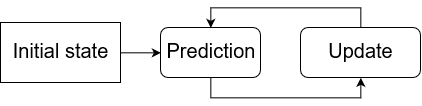
\includegraphics[width=0.5\textwidth]{chapter2/images/kalmanProcess.png}
		\caption{ผังการทำงานของระบบติดตามการเคลื่อนไหวของวัตถุแบบ kalman filter}
    	\label{fig:kalman_concept}
\end{figure}

ซึ่งในแต่ละช่วงการทำงานนั้นจะมีรายละเอียดดังนี้
\begin{enumerate}
	\setlength\itemsep{-0.25em}
	\item Initialize ในขั้นตอนนี้จะเป็นการกำหนดค่าเริ่มต้นให้กับเมทริกซ์สถานะหรือ state (x) และเมทริกซ์ความแปรปรวนหรือ covariance matrix (P) โดยที่เมทริกซ์สถานะจะใช้ในการเก็บข้อมูลที่ต้องการติดตามการเคลื่อนไหว 
	และเมทริกซ์ความแปรปรวนเป็นเมทริกซ์ที่ใช้บอกความแม่นยำของการทำนาย หากสามารถกำหนดค่าในเมทริกซ์ได้อย่างเหมาะสมจะทำให้การปรับปรุงประสิทธิภาพของ kalman filter ในช่วง update เสถียรเร็วขึ้น
	หากสมมติว่าสามารถหาตำแหน่งจุดกึ่งกลางของวัตถุในเฟรมแรกได้จะสามารถเขียนเมทริกซ์สถานะ และเมทริกซ์ความแปรปรวนได้ดังนี้
	\begin{equation*}
		x_0 = [c_x\ c_y\ v_x\ v_y]^T
	\end{equation*}
	\begin{equation*}
		P_0 = \begin{bmatrix}
			1& 0& 0& 0\\
			0& 1& 0& 0\\
			0& 0& 1& 0\\
			0& 0& 0& 1
			\end{bmatrix}
	\end{equation*}
	โดยที่ 
	\begin{conditions}
		x_0		&	เมทริกซ์สถานะ ณ เฟรมแรก\\
		c		&	จุดกึ่งกลางของวัตถุในภาพ\\
		v		&	ความเร็วในแกนที่กำหนด\\
		P_0		&	เมทริกซ์ความแปรปรวน ณ เฟรมแรก
	\end{conditions}
	จากตัวอย่างด้านบนจะเห็นว่าสิ่งที่สนใจนั้นเป็นตัวแหน่งของวัตถุ $(c_x, c_y)$ แต่ลำพังเพียงแค่ตำแหน่งไม่สามารถใช้ในการบอกตำแหน่งถัดไปได้จึงจำเป็นต้องมีข้อมูลเพิ่มเข้ามา 
	ซึ่งในที่นี้คือความเร็วในแต่ละแกน $(v_x, v_y)$ และได้กำหนดเมทริกซ์ความแปรปรวน ให้เป็น 1 ทั้งหมดไว้ก่อน (สามารถกำหนดเป็นเท่าไหร่ก็ได้ขึ้นอยู่กับระบบที่ต้องการติดตาม)
	\item Prediction ในขั้นตอนนี้จะเป็นการทำนายตำแหน่งหรือเมทริกซ์สถานะ $(x)$ และปรับเมทริกซ์ความแปรปรวน $(P)$ โดยใช้ข้อมูลจากเฟรมก่อนหน้าเป็นพื้นฐานในการคำนวณ 
	ซึ่งมีสมการดังนี้ 
	\begin{equation}
		x' = Fx + u
		\label{equa:estimate_state}
	\end{equation}
	\begin{equation}
		P' = FPF^T + Q
	\end{equation}
	โดยที่
	\begin{conditions}
		x'		&	state ถัดไปที่ได้จากการทำนาย\\
		F		&	state transition matrix\\
		u		&	แรงกระทำจากภายนอก (extermal force)\\
		Q		&	เมทริกซ์ความแปรปรวนที่สอดคล้องกับข้อมูลรบกวนของสถานะ (process covariance matrix)
	\end{conditions}
	จากสมการที่ \ref{equa:estimate_state} ตัวแปร $u$ หรือแรงกระทำจากภายนอกนั้นไม่สามารถหาได้จากภาพทำให้สามารถตัดออกไปได้ จะทำให้เหลือเพียง $x' = Fx$ ซึ่งตัวแปร $F$
	คือ เมทริกซ์ปรับสถานะ (state transition matrix) ซึ่งสามารถกำหนดได้เองขึ้นอยู่กับความต้องการของผู้พัฒนาโดยจะต้องสอดคล้องกับเมทริกซ์สถานะที่กำหนดไว้ สามารถเขียนตัวอย่างของเมทริกซ์ $F$ ได้ดังนี้
	\begin{equation*}
		F = \begin{bmatrix}
			1& 0& dt& 0\\
			0& 1& 0& dt\\
			0& 0& 1& 0\\
			0& 0& 0& 1
		\end{bmatrix}
	\end{equation*}
	โดย $dt$ หมายถึงความต่างของเวลาจากเฟรมก่อนหน้าถึงเฟรมปัจจุบัน จากตัวอย่างเมทริกซ์ $F$ ด้านบนนั้นเกิดจากการที่คาดว่าความเร็วในการเคลื่อนไหวของวัตถุนั้นคงที่ 
	เนื่องจากการกำหนดเมทริกซ์ $F$ ให้เป็น 1 นั้นถ้าหากนำเมทริกซ์ $F$ ไปคูณกับเวกเตอร์ $x$ จะทำให้ได้ตำแหน่งต่อไปที่เกิดจากการคำนวณ หรือ $x'$
	\begin{equation*}
		x' = \begin{bmatrix}
			1& 0& dt& 0\\
			0& 1& 0& dt\\
			0& 0& 1& 0\\
			0& 0& 0& 1
		\end{bmatrix} \begin{bmatrix}
			c_x\\ c_y\\ v_x\\ v_y
		\end{bmatrix} = \begin{bmatrix}
			c_x + v_xdt\\ c_y + v_ydt\\ v_x\\ v_y
		\end{bmatrix}
	\end{equation*}
	จากนั้นจะทำการคำนวณหาเมทริกซ์ความแปรปรวนในเวลาถัดไป ($P'$) โดยใช้เมทริกซ์ $Q$ ที่เป็นเมทริกซ์ความแปรปรวนที่สอดคล้องกับข้อมูลรบกวนของสถานะในการปรับประสิทธิภาพของการทำนายสถานะถัดไปของวัตถุ 
	ซึ่งมักจะถูกกำหนดให้เป็นเมทริกซ์เอกลักษณ์ (identity matrix) ที่มีขนาดเท่ากันกับเมทริกซ์ $P$ ทั้งนี้ก็ขึ้นอยู่กับระบบของผู้ใช้
	\item Update ในขั้นตอนนี้จะเกิดขึ้ยหลังจากมีการวัดค่า (measurement) ครั้งใหม่เข้ามาเพื่อนำข้อมูลที่ได้จากการวัดค่ามาเทียบกับข้อมูลที่ได้จากขั้นตอน prediction เพื่อคำนวณหาความคลาดเคลื่อน 
	และปรับตัวแปรต่างๆให้มีความเสถียรมากขึ้น โดยมีจะมีการคำนวณหาเมทริกซ์สถานะและเมทริกซ์ความแปรปรวนที่ผ่านการปรับแล้วด้วยสมการดังนี้
	\begin{equation}
		x = x' + Ky
		\label{equa:new_state}
	\end{equation}
	\begin{equation}
		P = (I-KH)P'
		\label{equa:new_covariance}
	\end{equation}
	จากสมการที่ \ref{equa:new_state} ตัวแปร $y$ คือค่าความคลาดเคลื่อนระหว่างสถานะที่ได้จากการวัดค่ามา ($z$) กับสถานะที่ทำนายมา 
	หากเป็นการติดตามการเคลื่อนไหวของวัตถุในวิดีโอนั้นสิ่งที่สามารถวัดออกมาได้มักจะเป็นตำแหน่งของวัตถุ สามารถเขียนได้ว่า $z=[c_x\ c_y]^T$ ซึ่งมีมิติไม่เท่ากันกับเมทริกซ์ $x'$ 
	จึงจำเป็นต้องมีเมทริกซ์สำหรับปรับมิติ ($H$) สามารถเขียนเป็นสมการได้ดังนี้
	\begin{equation}
		y = z - Hx'
	\end{equation}
	เนื่องจาก $x'$ มีมิติเป็น 4x1 ในขณะที่ $z$ มีมิติเป็น 2x1 ทำให้เมทริกซ์ $H$ ต้องเป็นเมทริกซ์เอกลักษณ์ที่มีมิติเป็น 2x4 เพื่อปรับมิติของเมทริกซ์ $x'$ ให้เป็น 2x1 หลังจากได้ค่าความคลาดเคลื่อนแล้วก็ต้องหาค่า
	Kalman gain ($K$) โดยสามารถหาได้จากสมการดังนี้
	\begin{equation}
		K = P'H^TS^{-1}
	\end{equation}
	โดยที่เมทริกซ์ $S$ หาได้จากการนำเมทริกซ์ความแปรปรวนในเวลาถัดไป ($P'$) มารวมกับเมทริกซ์ของข้อมูลรบกวน (noise) โดยเมทริกซ์ของข้อมูลรบกวนนั้นผู้ใช้ต้องกำหนดขึ้นมาให้สอดคล้องกับระบบ 
	ซึ่งในที่นี้คือการเคลื่อนไหวของวัตถุในวิดีโอ ทำให้สามารถพิจารณาได้ว่าจะเกิดข้อมูลรบกวนบนตำแหน่งแกน $x$ และแกน $y$ โดยที่การเคลื่อนไหวในแนวแกน $x$ นั้นมีข้อมูลรบกวนมากกว่าในแนวแกน $y$ 
	ทำให้สามารถเขียนเมทริกซ์ $S$ และเมทริกซ์ข้อมูลรบกวน  ได้ดังนี้
	\begin{equation}
		S = HP'H^T + R
		\label{equa:Smatrix}
	\end{equation}
	\begin{equation*}
		R = \begin{bmatrix}
			4 & 0\\ 
			0 & 2
			\end{bmatrix}
	\end{equation*}
	จากสมการที่ \ref{equa:Smatrix} เนื่องจากเมทริกซ์ความคลาดเคลื่อน ($y$) มีมิติเป็น 2x1 ทำให้ Kalman gain ต้องมีมิติเป็น Nx2 เพื่อให้สามารถคูณกันกับเมทริกซ์ความคลาดเคลื่อนได้ โดยที่ N คือ
	จำนวนของสถานะที่สามารถวัดค่าได้ ในที่นี้สถานะที่สามารถวัดค่าได้มี 2 ตัวคือ $c_x$ และ $c_y$ ส่งผลให้เมทริกซ์ $S$ ต้องมีขนาดเป็น 2x2 เช่นกัน แต่เนื่องจากเมทริกซ์ $P'$ มีมิติเป็น 4x4 จึงต้องใช้เมทริกซ์ $H$ 
	ในการปรับมิติให้กลายเป็น 2x2 เพื่อที่จะสามารถรวมกันกับเมทริกซ์ของข้อมูลรบกวนได้
	\begin{equation}
		P = (I-KH)P'
	\end{equation}
\end{enumerate}
\begin{figure}[!ht]
	\centering
	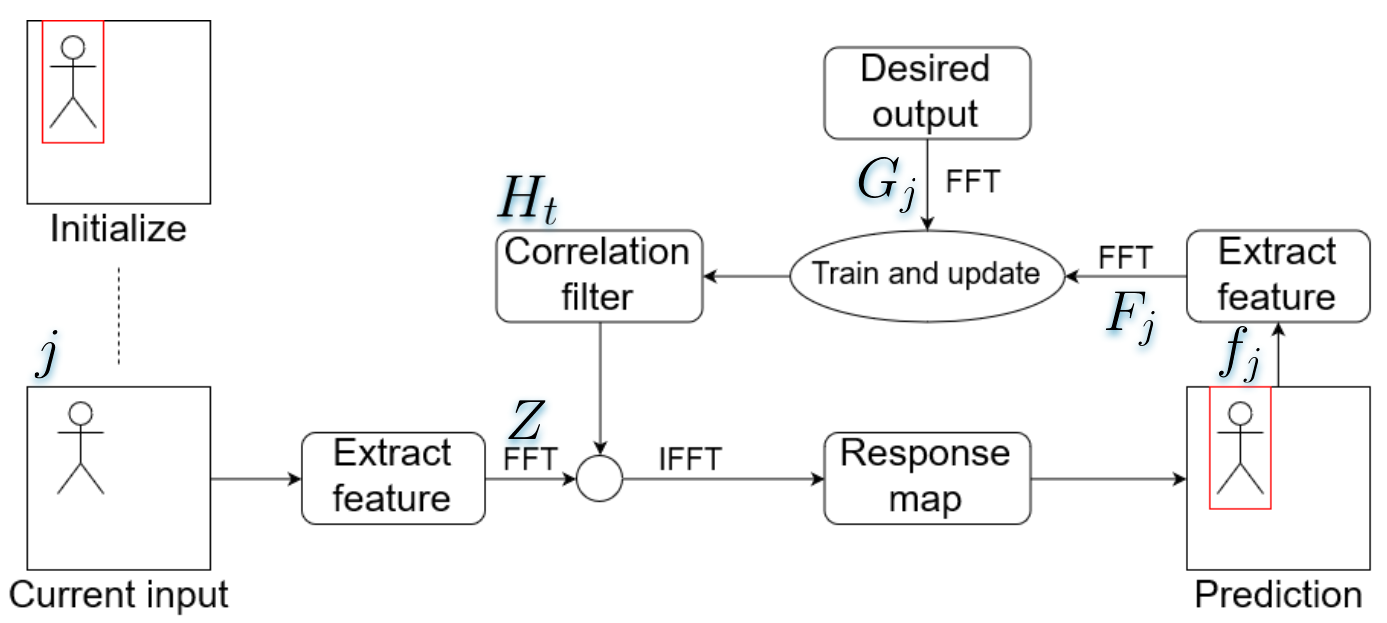
\includegraphics[width=1\textwidth]{chapter2/images/CorrelationTrack.png}
		\caption{ผังการทำงานของระบบติดตามการเคลื่อนไหวของวัตถุแบบ correlation filter}
    	\label{fig:correlation_concept}
\end{figure}

จากรูปที่ \ref{fig:correlation_concept} เป็นหลักการในการติดตามการเคลื่อนไหวของวัตถุแบบ correlation filter โดยการนำรูปมาผ่านกระบวนการแปลงฟูรีเยร์ (fourier transform)
และนำมาคูณกับ correlation filter ซึ่งเป็นตัวกรองที่ใช้สำหรับการหาความสัมพันธ์กับวัตถุในภาพ จากนั้นทำการแปลงฟูรีเยร์ผกผัน (inverse fourier transform) 
เพื่อตรวจสอบว่าวัตถุในภาพนั้นอยู่ที่ตำแหน่งใด โดยมีการคำนวณเริ่มจากการหา correlation filter ที่ดีที่สุดโดยใช้วิธีลดผลรวมของข้อผิดพลาดกำลังสองให้น้อยที่สุดดังนี้

\begin{equation}
\epsilon = \left \| \sum_{l = 1}^{d} h^{l} \star f^{l} - g \right \|^2 + \lambda \sum_{l = 1}^{d}\left \| h^{l} \right \|^2
\end{equation}
โดยที่
\begin{conditions}
 \epsilon     	&   ค่าความคลาดเคลื่อน 							\\
 d      		&  จำนวนมิติของผังคุณลักษณะของภาพ  \\   
 h 			&  correlation filter								\\
\star 			&  circular correlation							\\
 f			&  พื้นที่สี่เหลี่ยมของวัตถุที่สนใจที่ได้จากการทำผังคุณลักษณะ	\\
 g			&  ผลลัพธ์ correlation ที่ต้องการของ f					\\
 \lambda   		&  regularization term
\end{conditions}

เมื่อพิจารณาจากรูปภาพเดียวในกรณีที่เวลา ($t$) เท่ากับ 1 จะสามารถจัดรูปสมการด้านบนได้ดังนี้ 

\begin{equation}
H^{l} = \frac{\bar{G}F^{l}}{\sum_{k=1}^{d}\bar{F^{k}}F^{k} + \lambda}
\end{equation}
\begin{equation}
H_{t}^{l} = \frac{A_{t}^{l}}{B_{t}}					
\end{equation}					
\begin{equation}
A_{t}^{l} = (1-\eta )A_{t-1}^{l} + \eta \bar{G_{t}}F_{t}^{l}
\end{equation}
\begin{equation}
B_{t} = (1-\eta )B_{t-1} + \eta \sum_{k=1}^{d}\bar{F_{t}^{k}}F_{t}^{k}
\end{equation}
\clearpage
\noindent
โดยที่
\begin{conditions}
 H 		     	&   correlation filter								\\
 \eta      		&  อัตราการเรียนรู้						 		\\   
 \bar{G} 		&  g ที่ผ่านการทำ complex conjugation					\\
 F			&  พื้นที่สี่เหลี่ยมของวัตถุที่สนใจที่ได้จากการทำผังคุณลักษณะ	\\
 \bar{F}		&   f ที่ผ่านการทำ complex conjugation					\\
 t 	  		&  เวลา
\end{conditions}
จากสมการที่ได้มาจะสามารถทำให้หาตำแหน่งต่อไปของวัตถุที่สนใจได้ด้วยสมการต่อไปนี้
\begin{equation}
y = F^{-1}\left \{ \frac{\sum_{l = 1}^{d} \bar{A^{l}}Z^{l}}{B + \lambda} \right \}
\end{equation}
โดยที่
\begin{conditions}
 y 		     	&   correlation score										\\
 F^{-1}    		&  การแปลงฟูรีเยร์ผกผันแบบไม่ต่อเนื่อง (inverse discrete fourier transform)						\\   	
 \bar{A}^{l} 	&  $A^{l}$ ที่ผ่านการทำ complex conjugation				\\
 Z	 		&  พื้นที่สี่เหลี่ยมของวัตถุที่สนใจที่ได้จากการหาผังคุณลักษณะของภาพใหม่	
\end{conditions}
โดยค่าของ $y$ ที่ได้ออกมาจะทำให้รู้ถึงตำแหน่งของวัตถุที่สนใจได้ ณ ตำแหน่งที่ $y$ มีค่าสูงสุด